\question{Интеграл с переменным верхним пределом. Теорема Барроу.}

\begin{minipage}{\linewidth}
  \begin{multicols*}{2}
  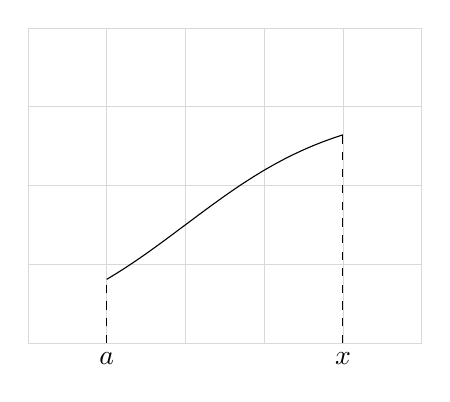
\begin{tikzpicture}
  \draw[very thin, gray!30, step = 1cm] (0, 0) grid (5, 4);
  \draw[domain = 1 : 4, variable = \x]
    plot ({\x}, {3 / (1 + e^(2 - \x))});

  \draw[dashed] (1, 0) -- (1, 0.807);
  \draw[dashed] (4, 0) -- (4, 2.642);
  \draw node[below] at (1, 0) {\(a\)};
  \draw node[below] at (4, 0) {\(x\)};
\end{tikzpicture}

  \columnbreak

  \begin{definition}
    Интегралом с переменных верхним пределом называется
    
    \begin{align*}
      \int_{a}^{x} f(t) \dd t
    \end{align*}

    где \(x\)~--- переменный верхний предел.
  \end{definition}
  \end{multicols*}
\end{minipage}

\begin{remark}
  \(\forall x \in [a; +\infty]\) соответствует определенное значение
  \(\Phi(x) = \int_{a}^{x} f(t) \dd t\), т.е. определена функция верхнего
  предела, которая геометрически является площадью криволинейной трапеции
  с подвижным правым краем.
\end{remark}

\begin{theorem}\label{Barrow}
  Теорема Барроу

  Пусть \(f \in C_{[a; b]}\) и определен \(\Phi(x) = \int_{a}^{x} f(t) \dd t\).
  Тогда \(\Phi'(x) = f(x)\).
\end{theorem}
\begin{proof}
  Раскроем производную \(\Phi'(x)\) по определению, после чего воспользуемся
  линейностью интеграла:

  \begin{align*}
    \Phi'(x)
    = \lim_{\Delta x \to 0} \frac{\Phi(x + \Delta x) - \Phi(x)}{\Delta x}
    = \lim_{\Delta x \to 0} \frac{
      \int_{a}^{x + \Delta x} f(t) \dd t - \int_{a}^{x} f(t) \dd t
    }{\Delta x}
    = \lim_{\Delta x \to 0} \frac{\int_{x}^{x + \Delta x} f(t) \dd t}{\Delta x}
  \end{align*}

  Далее по т. Лагранжа (\ref{L-mid-int}) \(\exists \xi \in (a; b)\) такая, что:

  \begin{align*}
    \lim_{\Delta x \to 0} \frac{\int_{x}^{x + \Delta x} f(t) \dd t}{\Delta x}
    = \lim_{\Delta x \to 0} \frac{f(\xi) \Delta x}{\Delta x}
    = \begin{bmatrix}
      \begin{rcases}
        \Delta x \to 0 \\
        \xi \in (x, x + \Delta x)
      \end{rcases}
      \implies \xi \to x
    \end{bmatrix}
    = f(x)
  \end{align*}
\end{proof}